% !TEX root =  ../report.tex
\graphicspath{{huereport/content/images/}}

\section{CONCLUSIONS \& IMPROVEMENTS}
\subsection{IMPROVEMENTS}
After conducting the heuristic usability evaluation, we identified areas for improvement in the application. The following sections describe the changes we recommend to enhance the overall user experience.
\newline
\newline
\indent To prioritize which problems should be addressed first, we evaluate them based on their severity and frequency. A matrix can be created with severity plotted horizontally and frequency vertically. The problems in the top left corner of the matrix, with high severity and frequency, should be addressed as soon as possible, while those in the bottom left corner, with low severity and frequency, can be considered last. 
\newline
\begin{figure}[H]
    \centering
    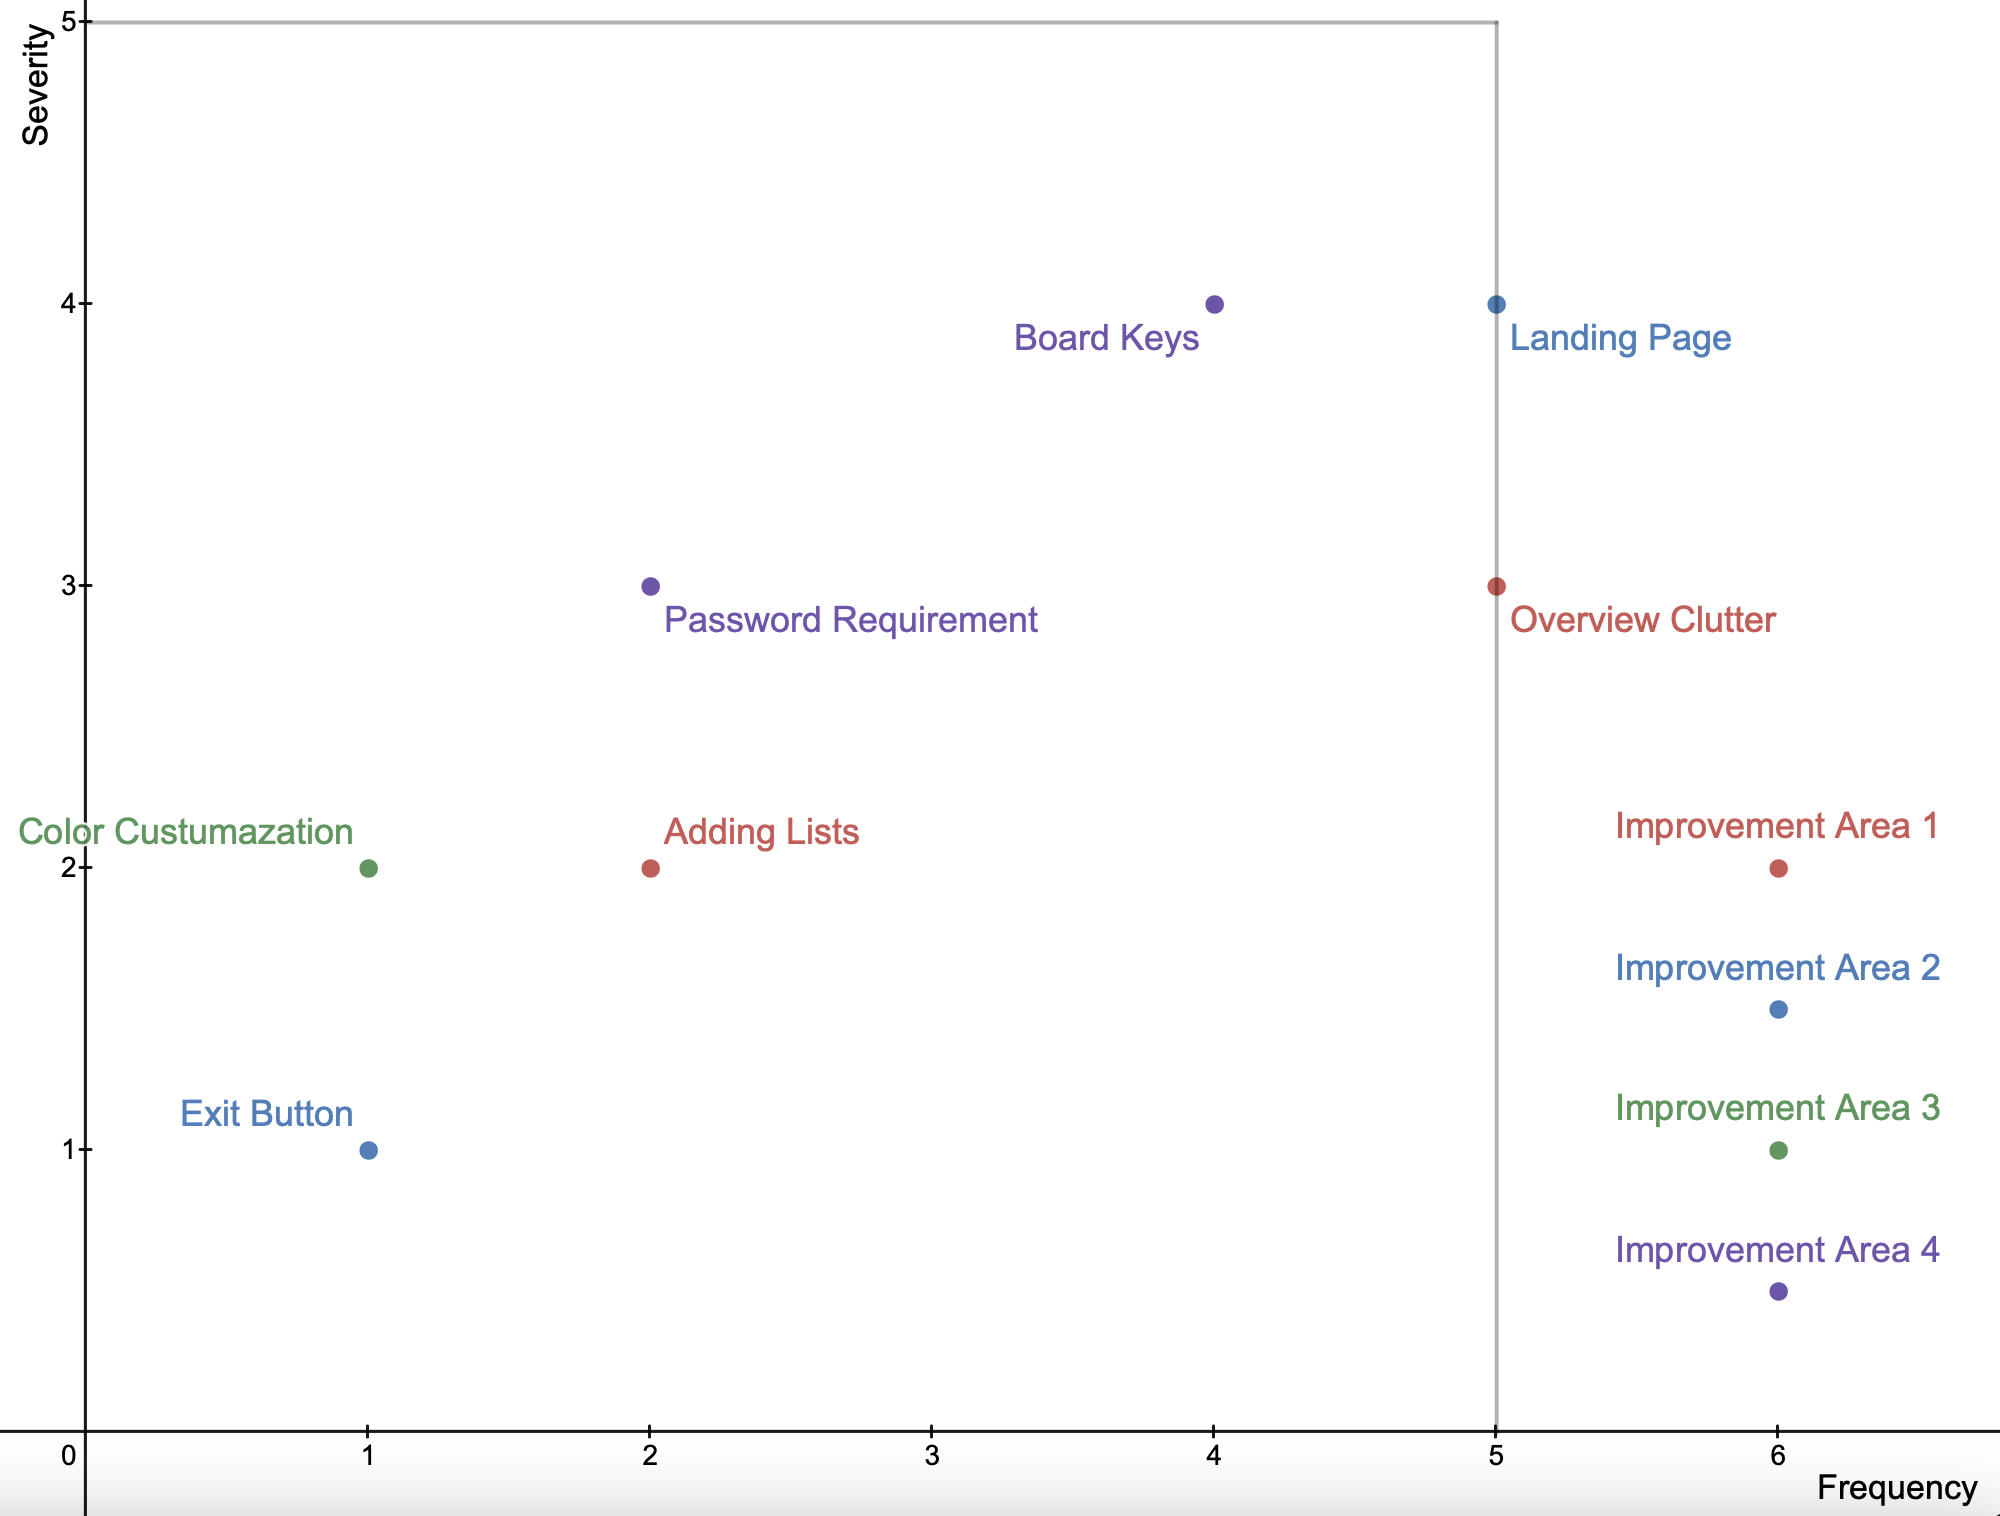
\includegraphics[width=0.5\textwidth]{eval-matrix.png}
    \caption{Severity × Frequency Matrix}
    \label{fig:matrix}
\end{figure}
\subsection*{Improvement Area 1: Board Overview Scene}
\indent The current design of the board overview scene suffers from two issues: clutter and poor button placement.
\newline\indent
To address these problems, the following changes have been proposed:
\newline\indent First, the add list button will be moved to the board sidebar, making it more accessible and prominent.
\newline 
\indent Second, the overall design will be simplified by removing card details from the board overview scene and creating a new card overview scene. Users can access the card overview by double-clicking on the card name. This separation of information between the two scenes will result in a more minimalist and user-friendly application. Following is the new design, approved by the developer team and reviewers.

\begin{figure}[H]
    \centering
    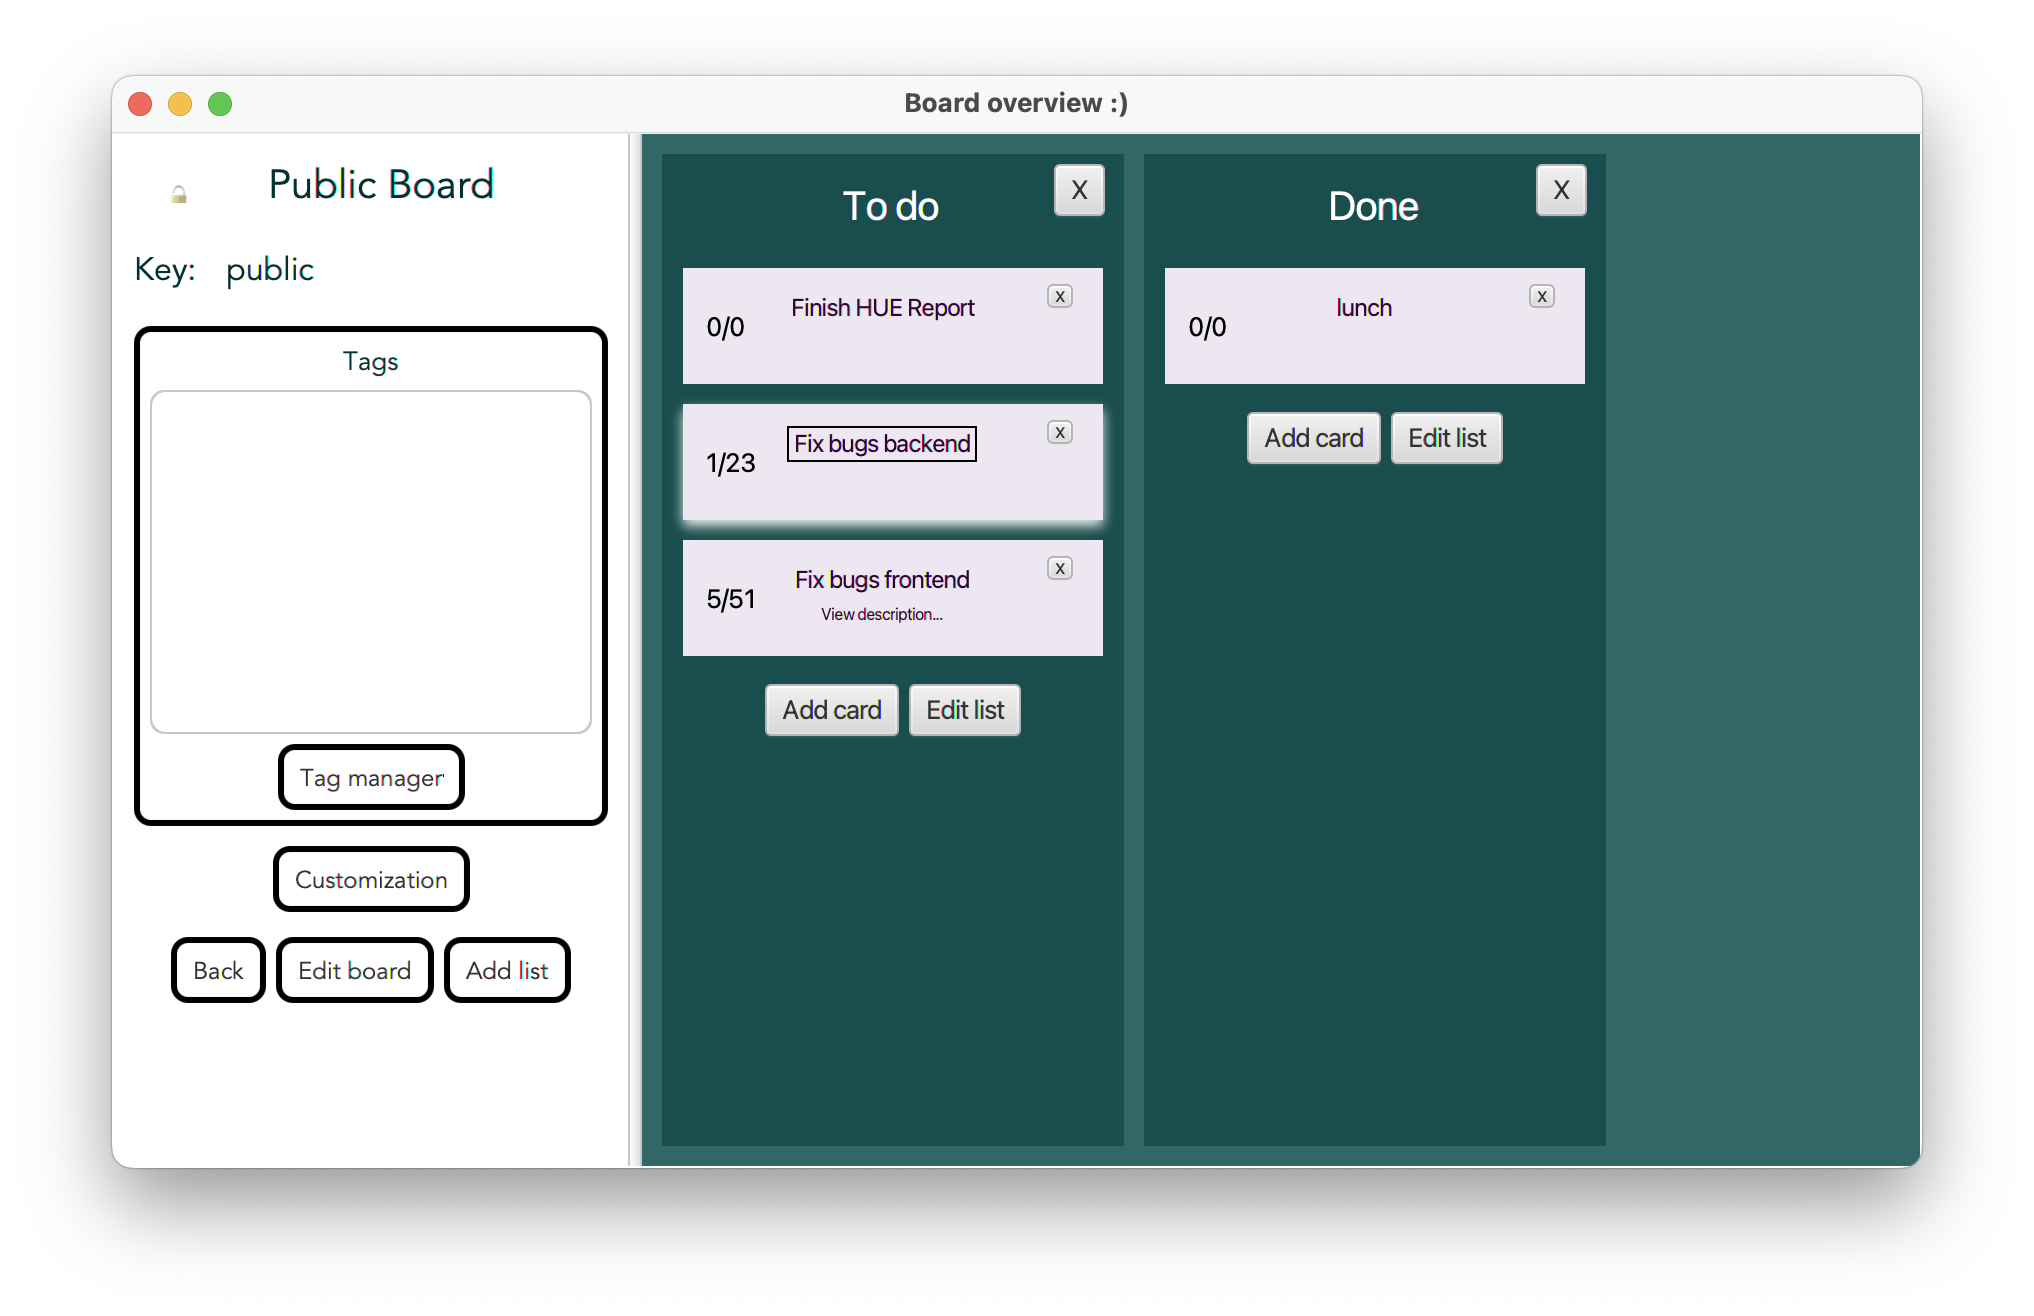
\includegraphics[width=0.47\textwidth]{new-overview.png}
    \caption{Redesigned Board Overview}
    \label{fig:overview-redesign}
\end{figure}


\subsection*{Improvement Area 2.}
\indent The Landing Page may be difficult to navigate for users without prior context or familiarity with the application.
\newline
\indent
This issue is addressed by completely redesigning the landing page. In the new design the page serves as the entry point to the application (replacing the server select scene as initial scene), directly offering help via a brief tutorial, and a button to switch to the select server scene. In future redesigns, the buttons on the Landing Page and subsequent pages could be styled with hover effects that provide more information on where each button will redirect the user.

\begin{figure}[H]
    \centering
    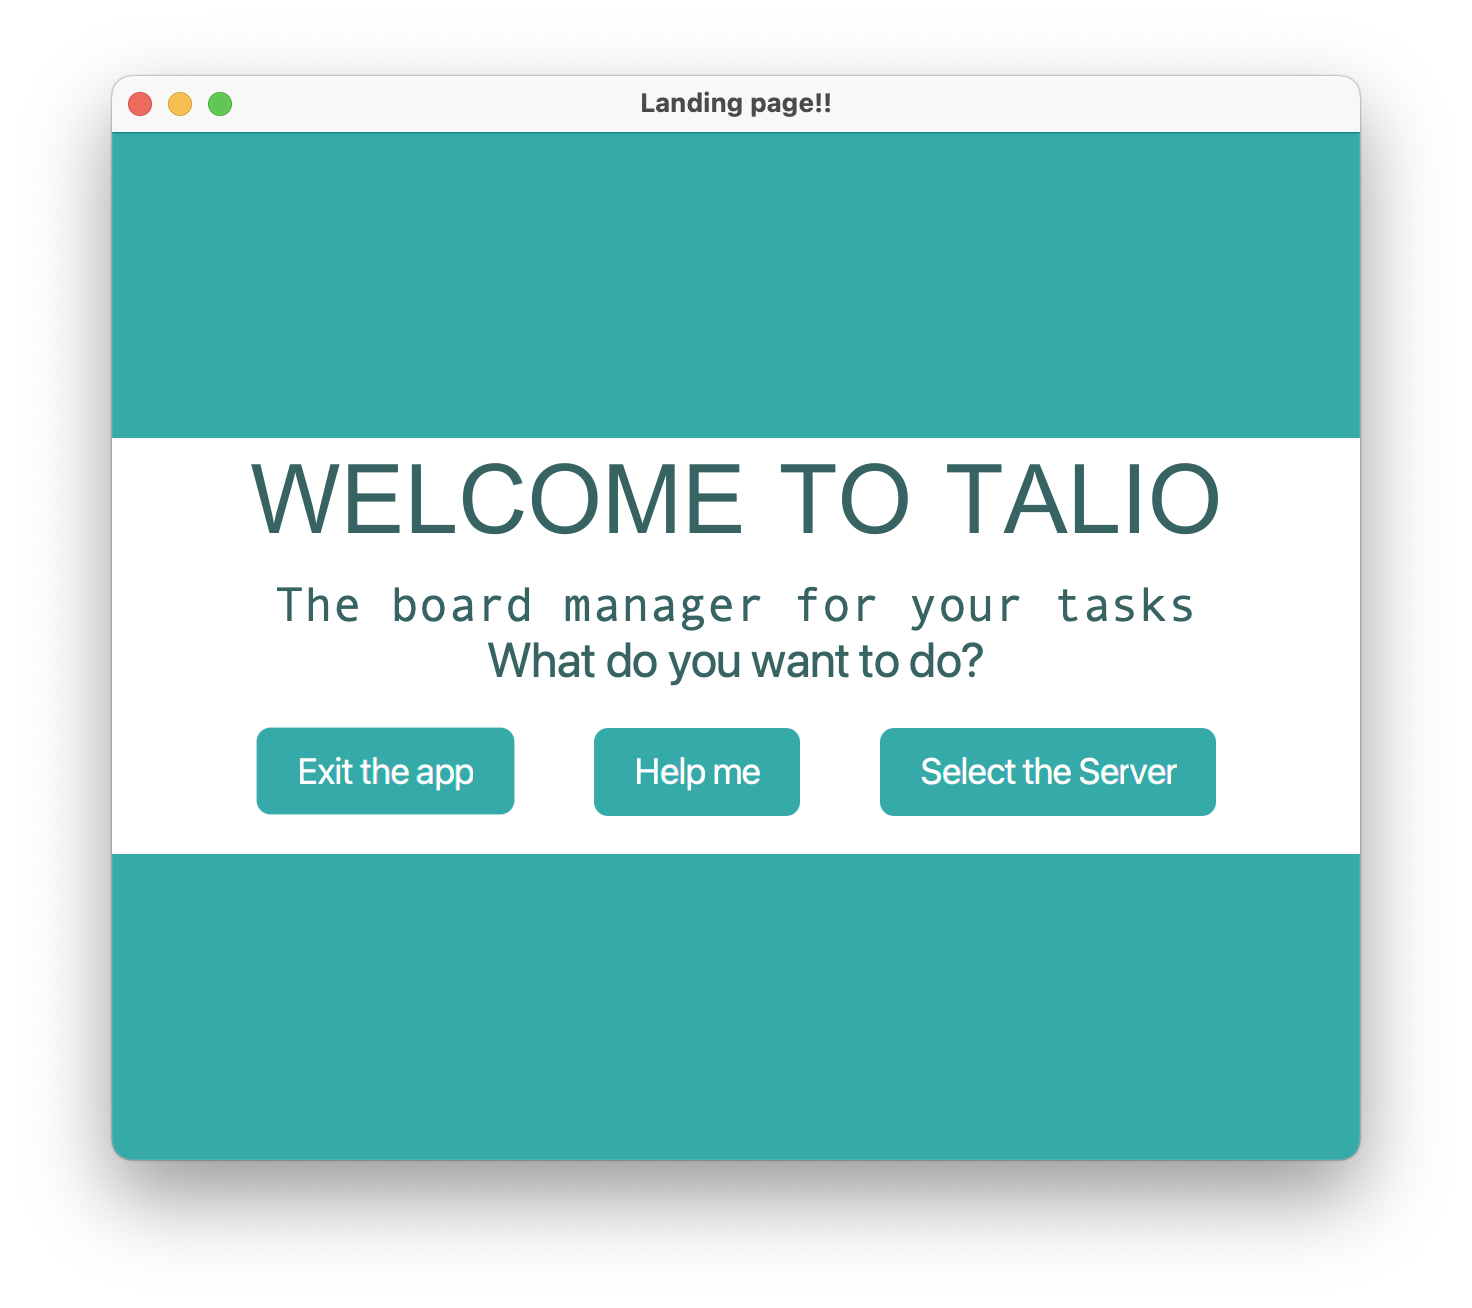
\includegraphics[width=0.4\textwidth]{landing-latest.png}
    \caption{Redesigned Landing Page}
    \label{fig:landing-redesign}
\end{figure}


\subsection*{Improvement Area 3.}
\indent Color customization is difficult to use. \newline\indent
To manage this, the developers decided on a separate
color management feature, where the user can decide on the board and lists color, and create specific palettes for the cards.

\begin{figure}[H]
    \centering
    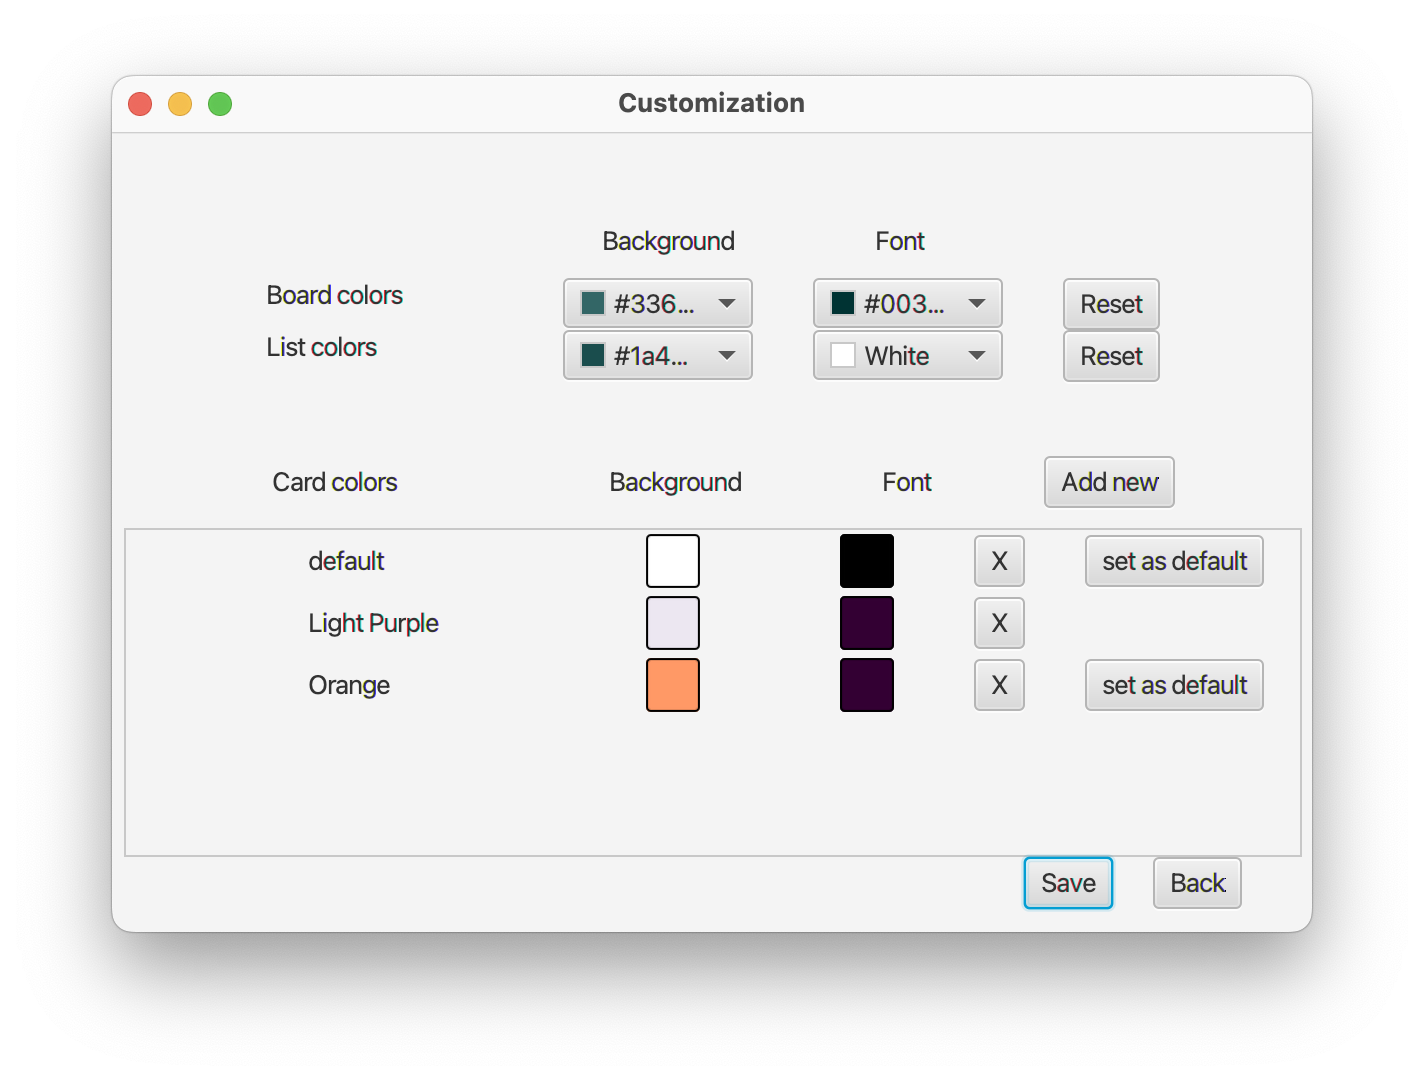
\includegraphics[width=0.47\textwidth]{customization.png}
    \caption{Colour Manager}
    \label{fig:colour-redesign}
\end{figure}

\subsection*{Improvement Area 4.}
\indent This area of the heuristic usability evaluation report identified two main issues with the board creation menu: the board key is confusing for new users, and the password system for the boards is inconsistent.
\newline
\indent One solution to the first issue is to change the text that refers to the board key to be more descriptive. Another proposed solution is to elaborate on the function of board keys in the help page.
\newline
\indent To address the second issue, the team decided to only opt the user to lock a board with a password within the board's overview page. This meant redesigning the board creation page to simply it as much as possible, moving optional functionality such as passwords and colours to later stages of the workflow.
\newline\indent
Following are the proposed design changes.
\begin{figure}[H]
    \centering
    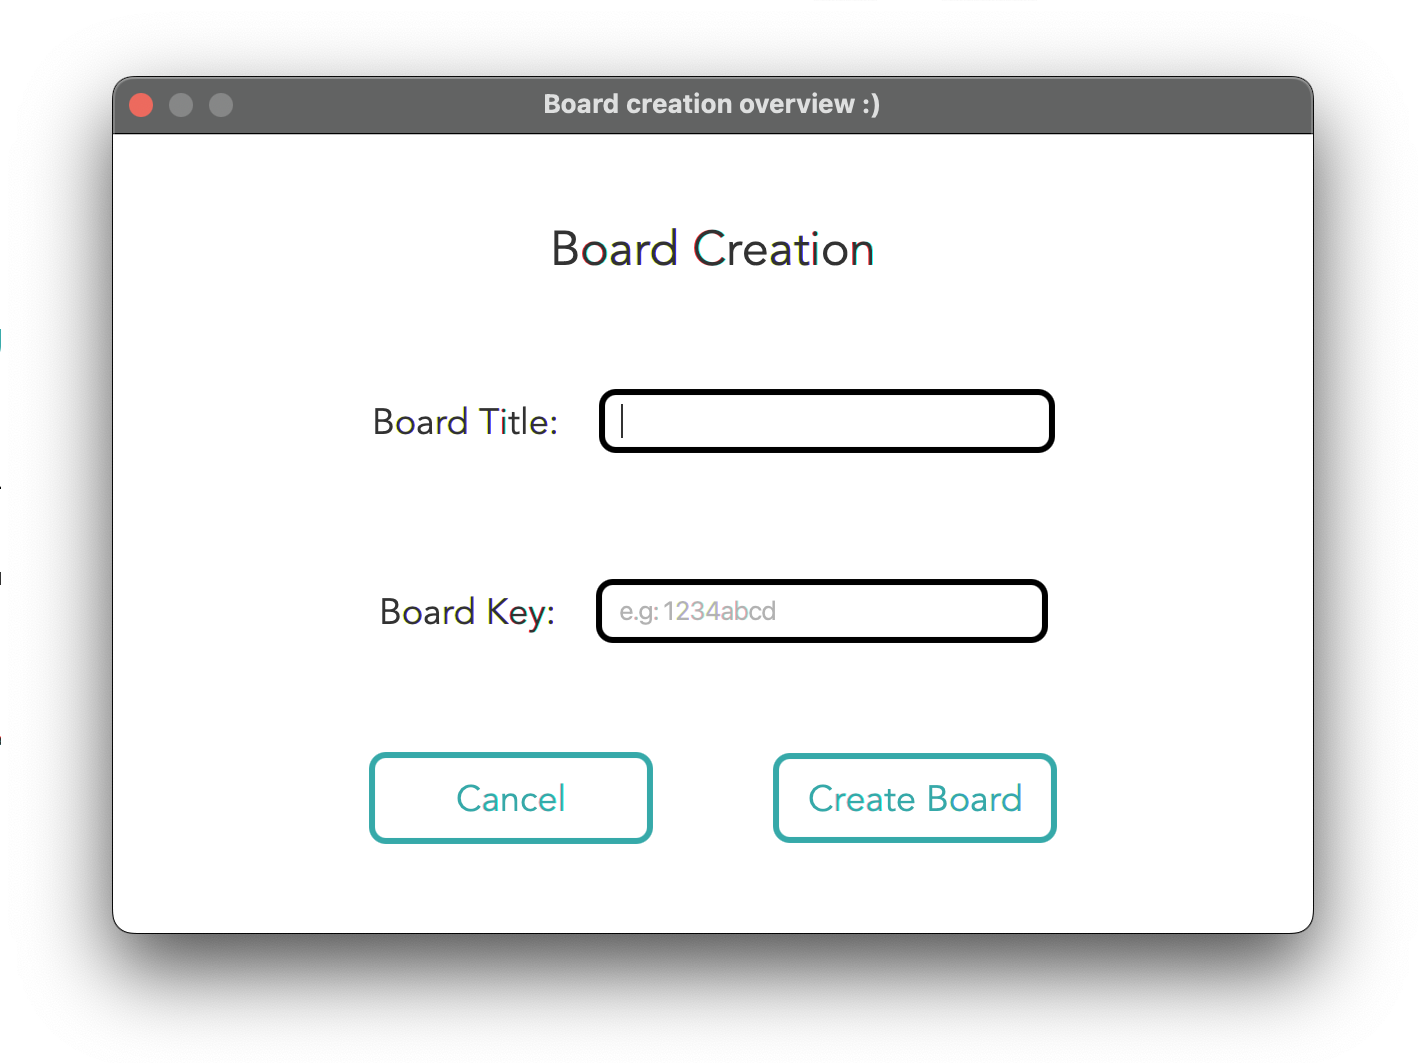
\includegraphics[width=0.47\textwidth]{create-board-2.png}
    \caption{New board Creation scene}
    \label{fig:board-create}
\end{figure}

\begin{figure}[H]
    \centering
    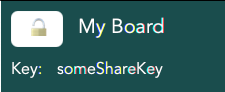
\includegraphics[width=0.175\textwidth, height=1.25cm]{lock-w.png}
    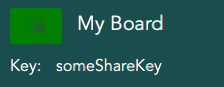
\includegraphics[width=0.175\textwidth, height=1.25cm]{lock-g.png}
    
\includegraphics[width=0.175\textwidth, height=1.1cm]{lock-r.png}
    \caption{Example of password protection.}
    \subsubsection*{Board with no password\newline Board with password, user has write access\newline Board with password, user has only read access to the content}
    \subsubsection*{}
    \label{fig:lock}
\end{figure}

\begin{figure}[H]
    \centering
    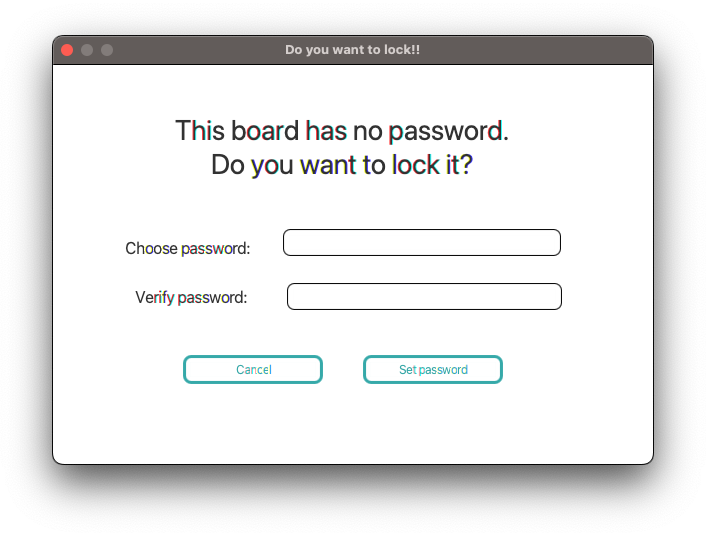
\includegraphics[width=0.47\textwidth]{add-pass.png}
    \caption{Example of setting a password. User can create a password and lock the board}
    \label{fig:set-pass}
\end{figure}

\begin{figure}[H]
    \centering
    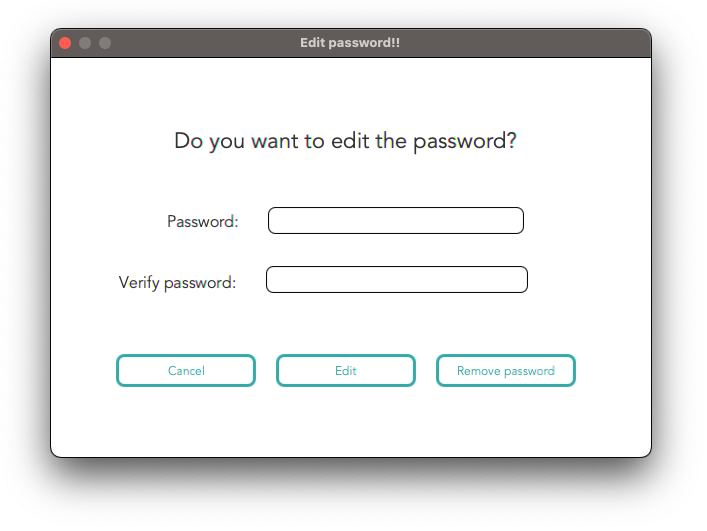
\includegraphics[width=0.47\textwidth]{edit-pass.png}
    \caption{Example of modifying a password. User can edit or remove it}
    \label{fig:edit-pass}
\end{figure}

\begin{figure}[H]
    \centering
    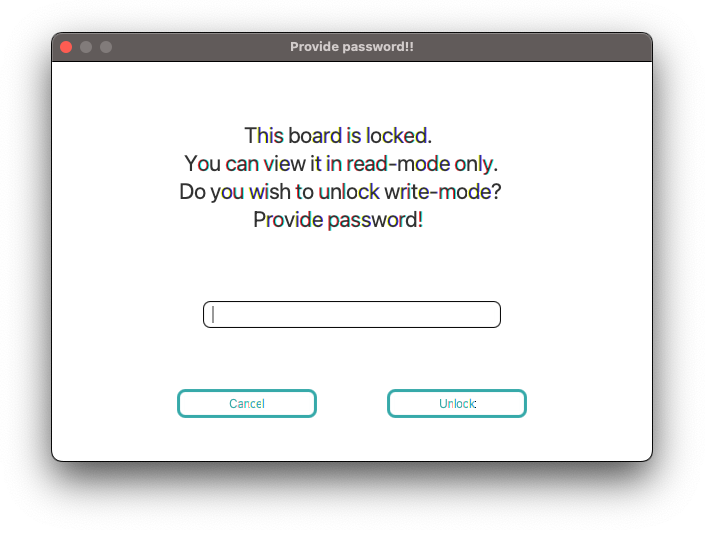
\includegraphics[width=0.47\textwidth]{unlock.png}
    \caption{Example of setting a password. User doesn't have access and is prompted to unlock the board}
    \label{fig:unlock-pass}
\end{figure}

